% !TEX TS-program = lualatex
% !TEX encoding = UTF-8

% This is a simple template for a LuaLaTeX document using gregorio scores.

\documentclass[letterpaper,12pt]{book} % use larger type; default would be 10pt

\input{header.inc}

\geometry{letterpaper,outer=0.4in,inner=0.9in,top=1in,bottom=0.8in}

\begin{document}
\printsmalltitle{Ave Virgo Serena}

\garamondbig
\greannotation{Seq.}
\greannotation{6.}
\gregorioscore{192_se--ave_mariavirgo_serena--solesmes}

\bigskip

\begin{centering}

\vfill

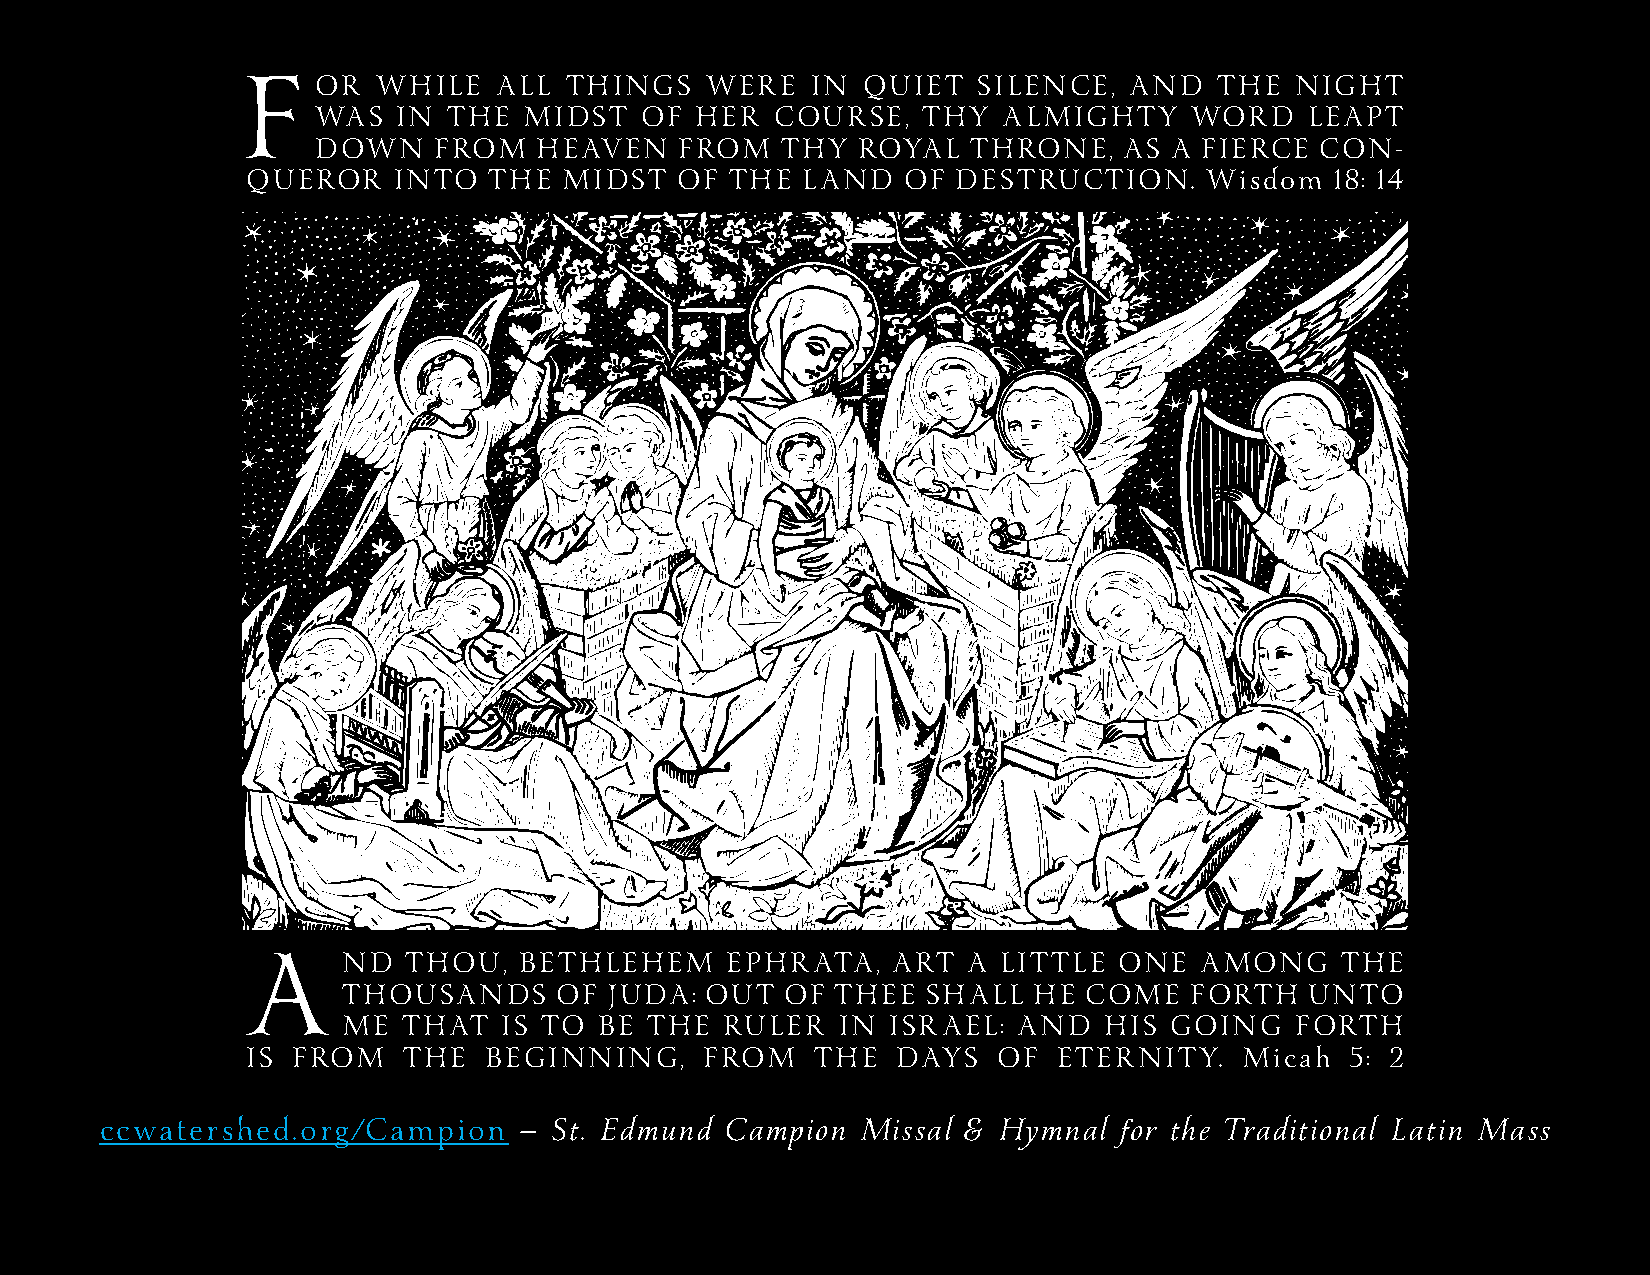
\includegraphics[clip,trim=1.615in 2.306in 1.616in 1.418in,width=.935\textwidth]{../195_clipart.pdf}

\vfill

\end{centering}

\pagebreak

\printsmalltitle{In honor of St.~Joseph}

\greannotation{Hymn.}
\greannotation{1.}
\gregorioscore{196_hy--caelitum_joseph_decus--solesmes}

\bigskip

\begin{centering}

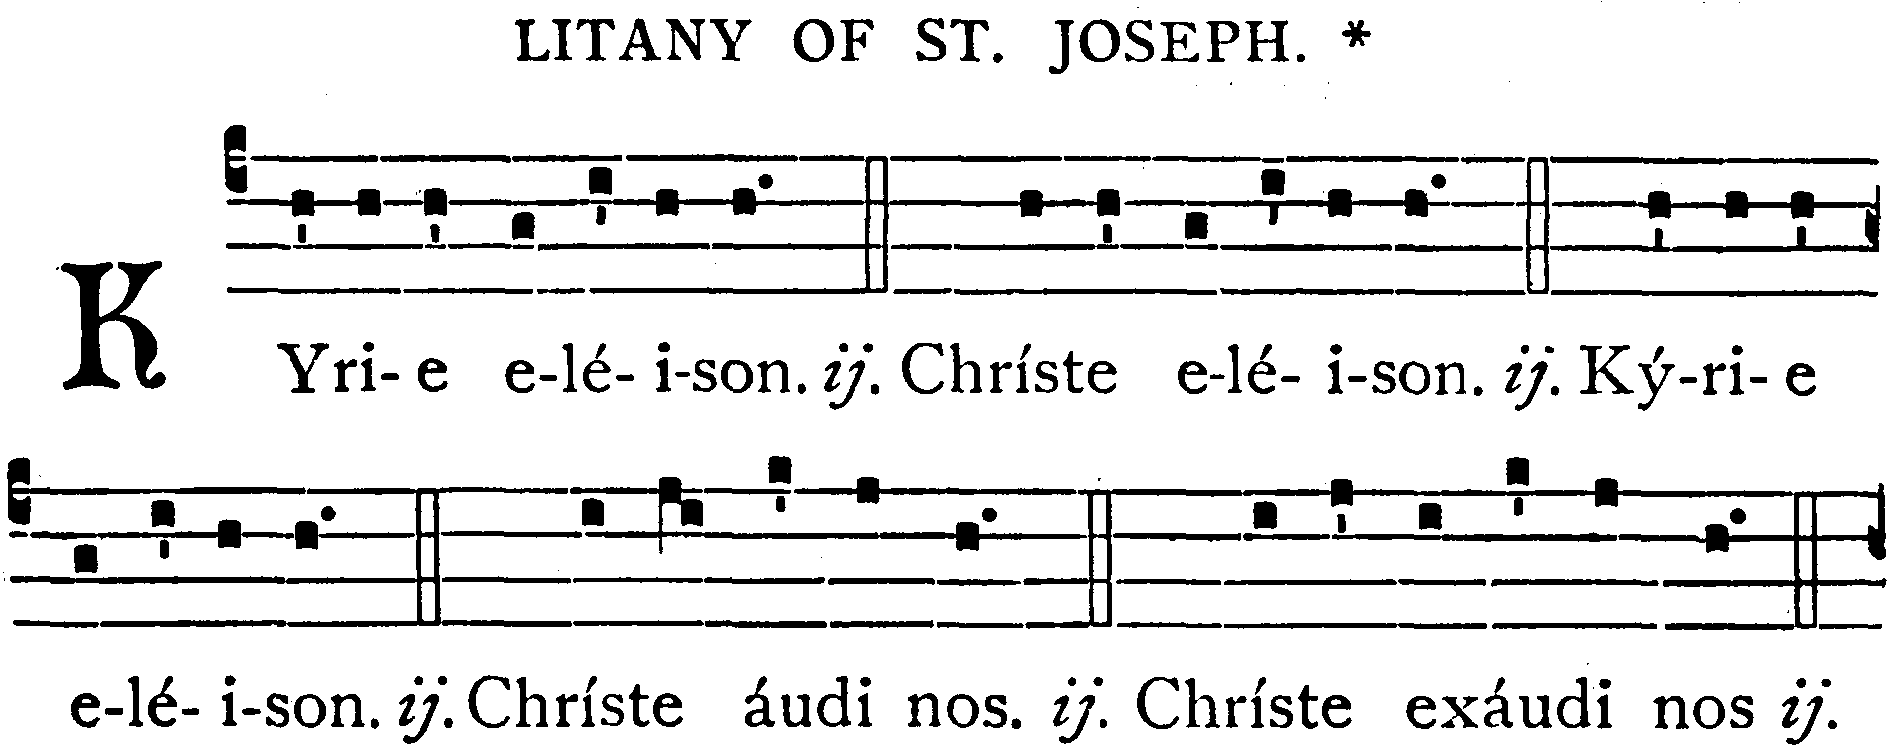
\includegraphics[width=\textwidth]{198-1.png}
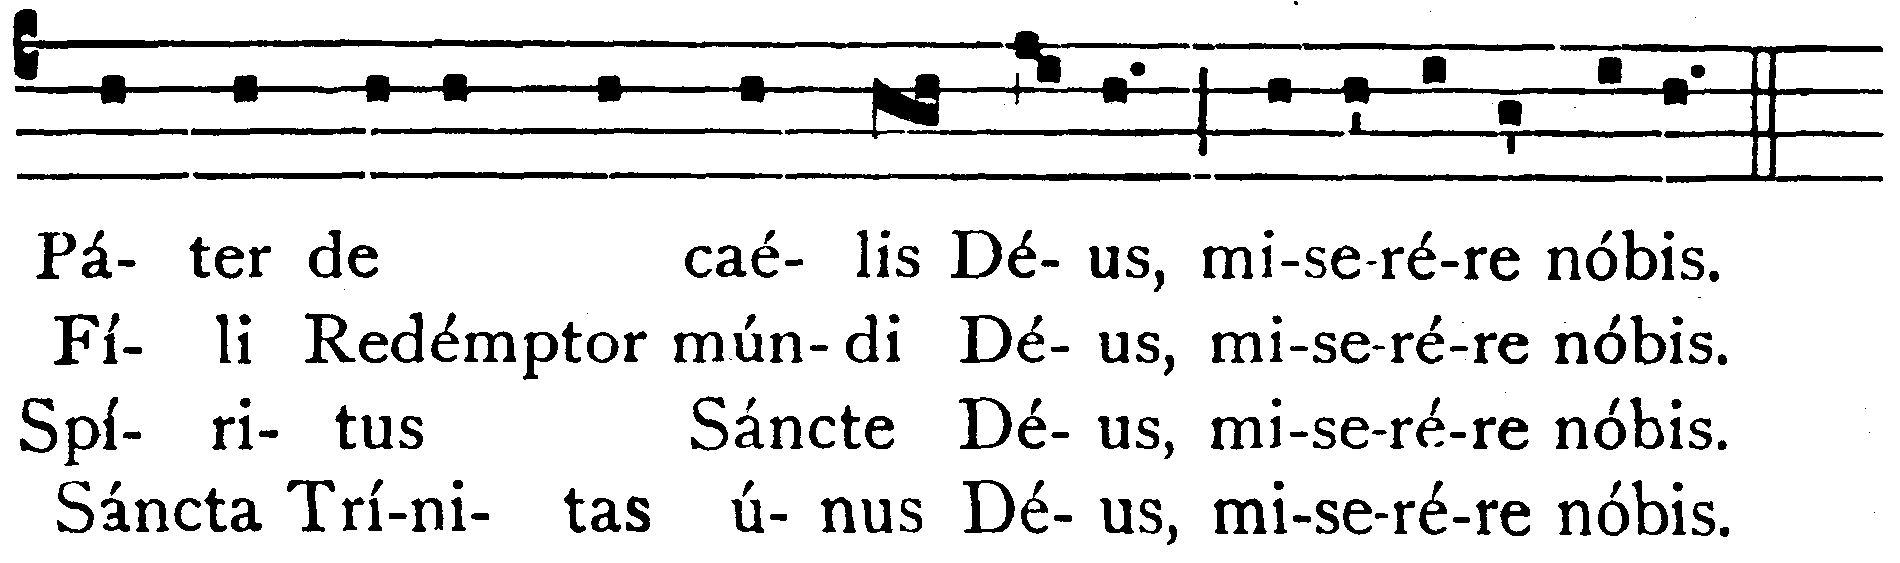
\includegraphics[width=\textwidth]{198-2.png}
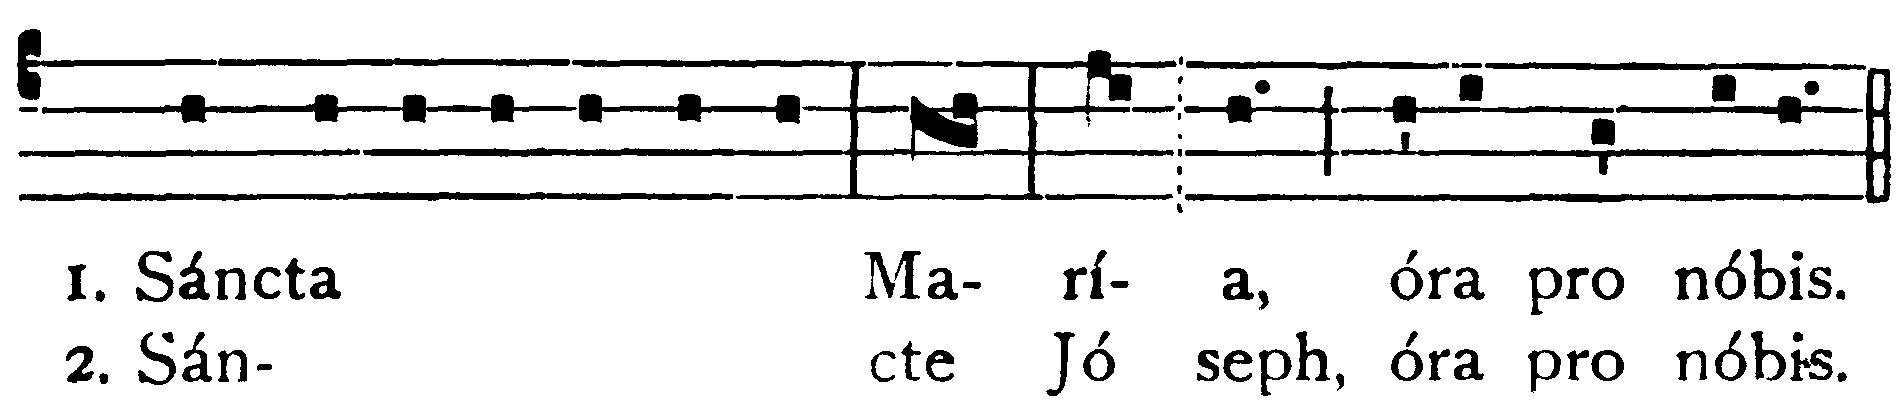
\includegraphics[width=\textwidth]{198-3.png}
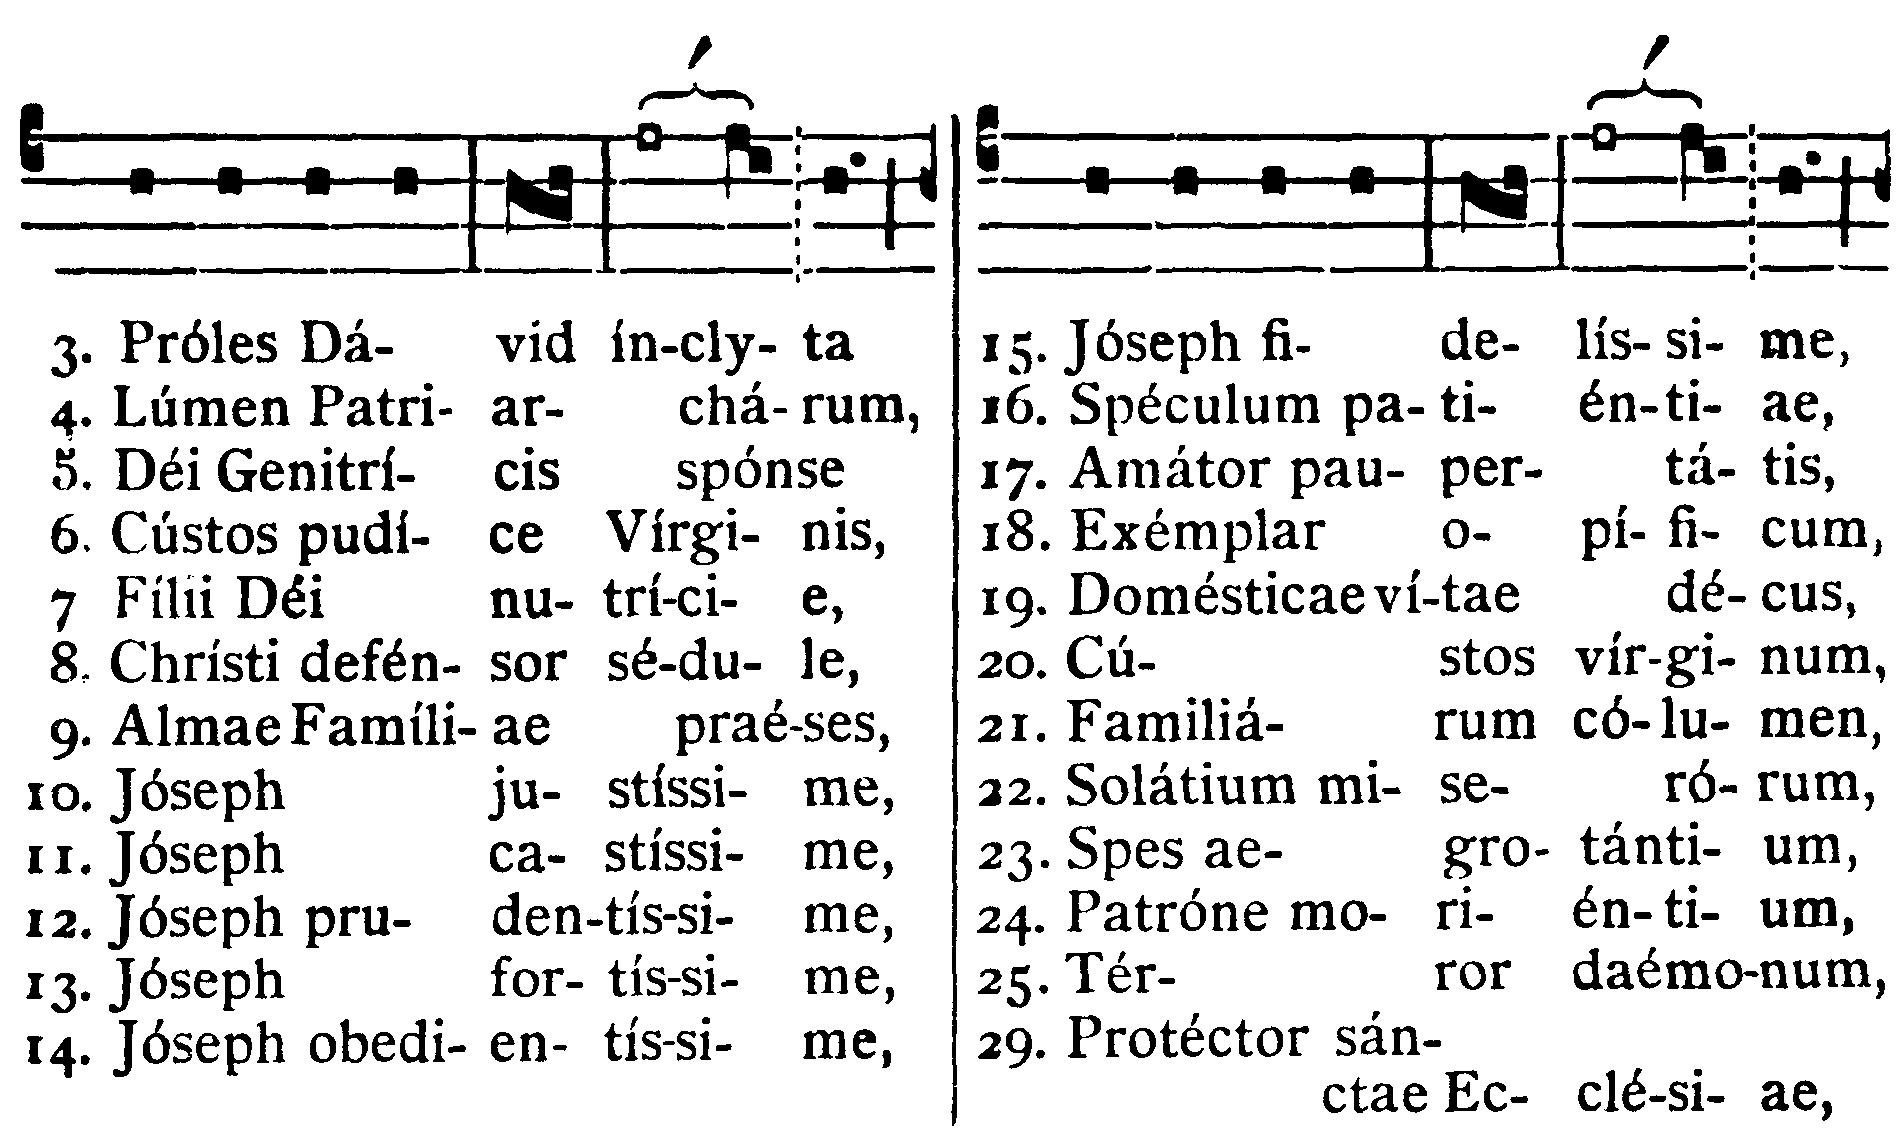
\includegraphics[width=\textwidth]{198-4.png}
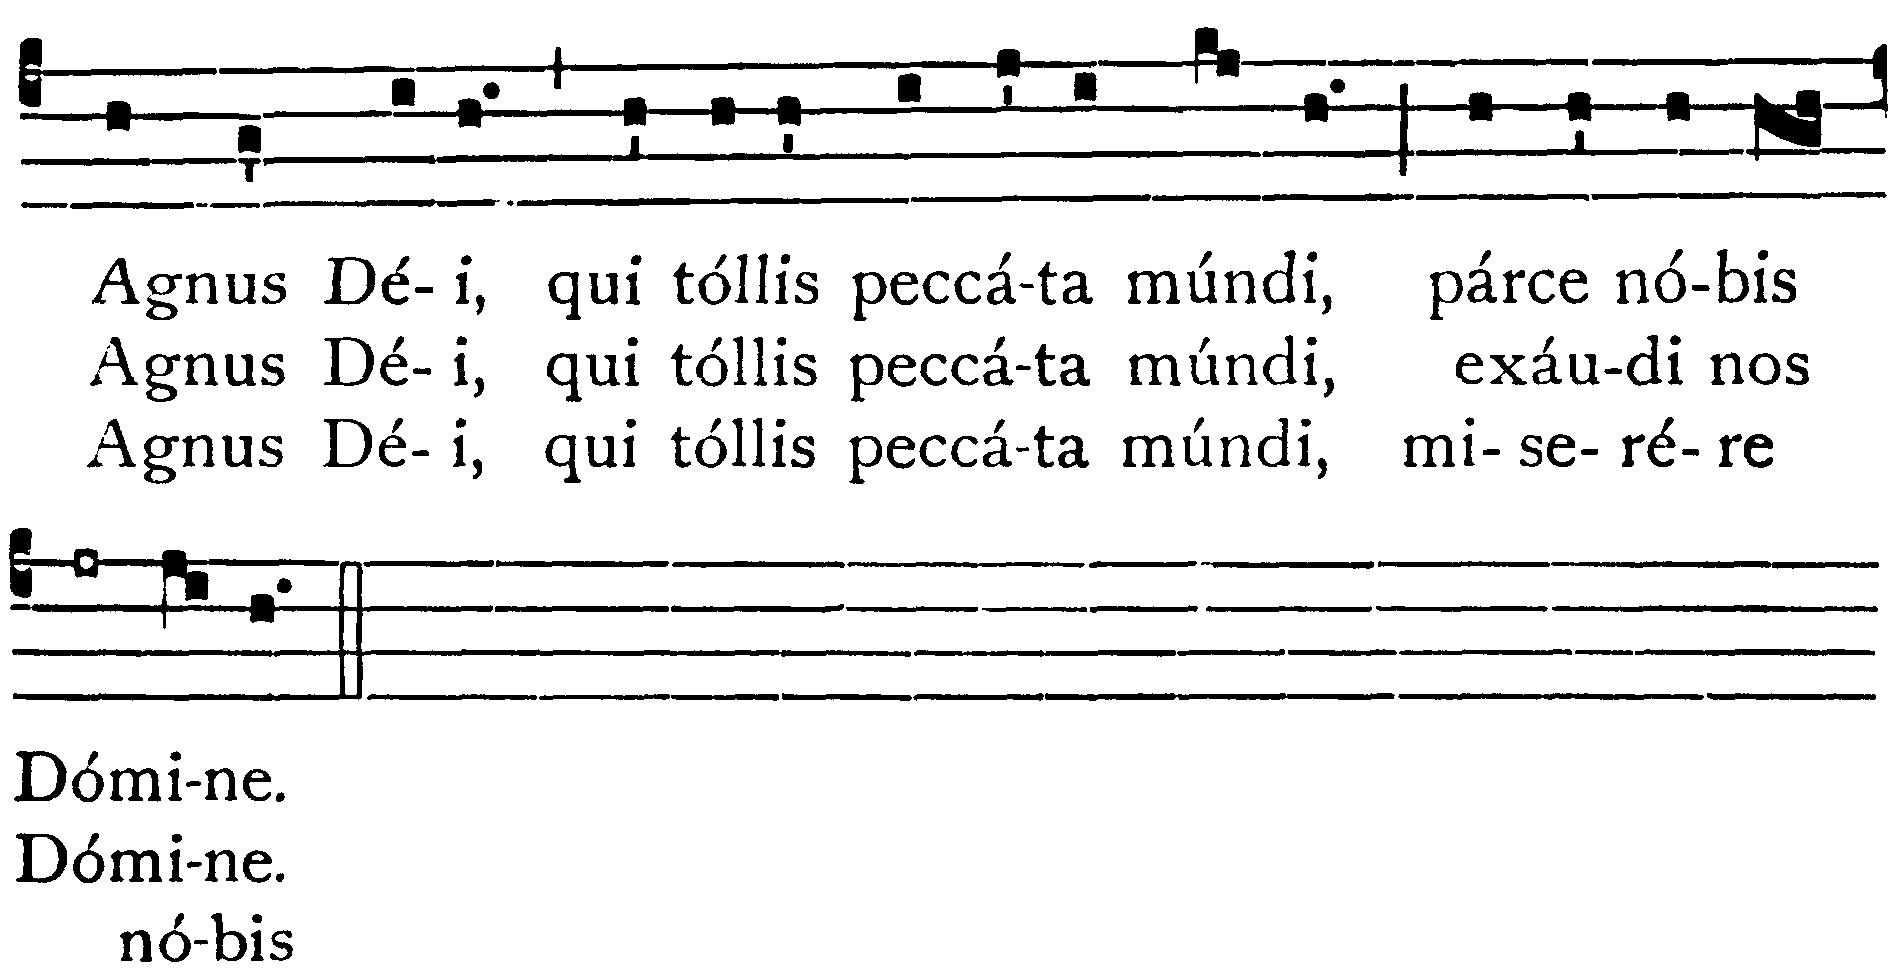
\includegraphics[width=\textwidth]{198-5.png}

\bigskip

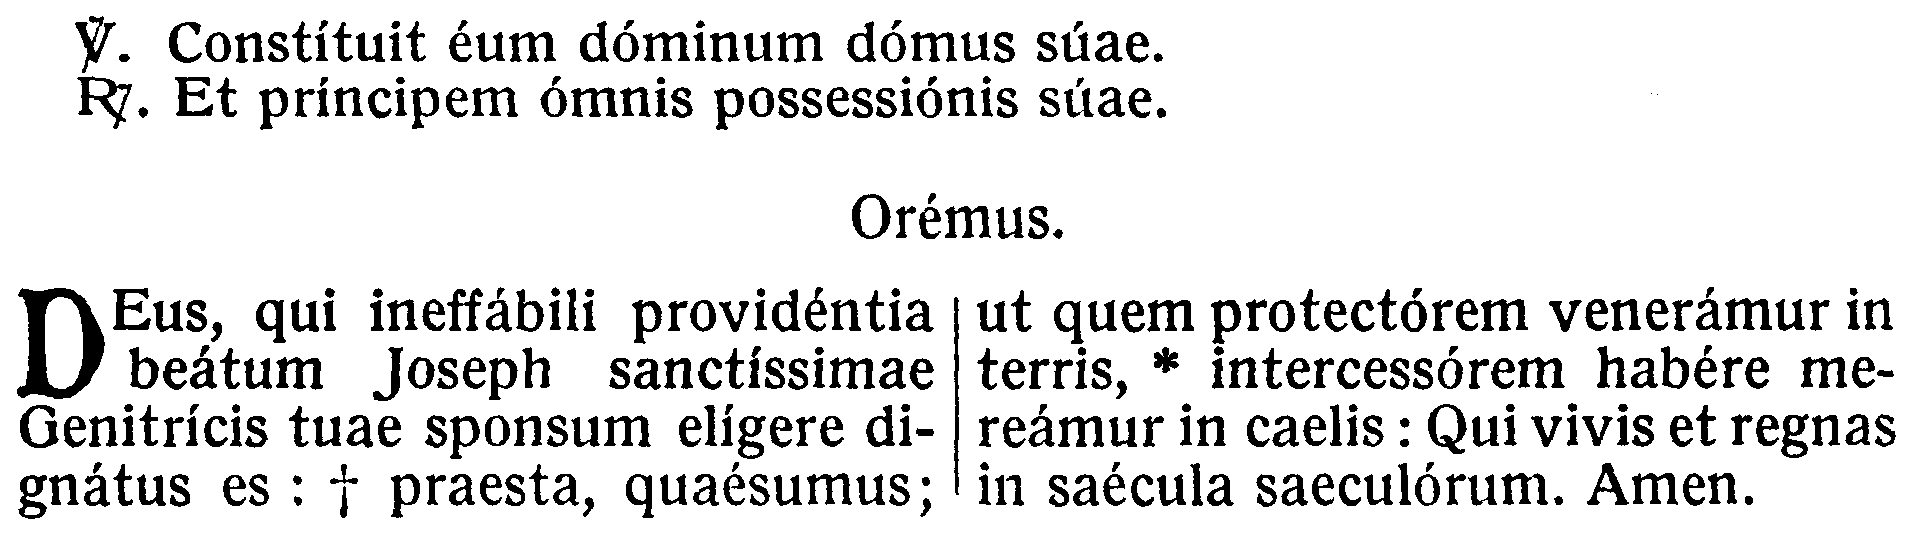
\includegraphics[width=\textwidth]{198-6.png}

\end{centering}

\bigskip
\begin{centering}

\vfill

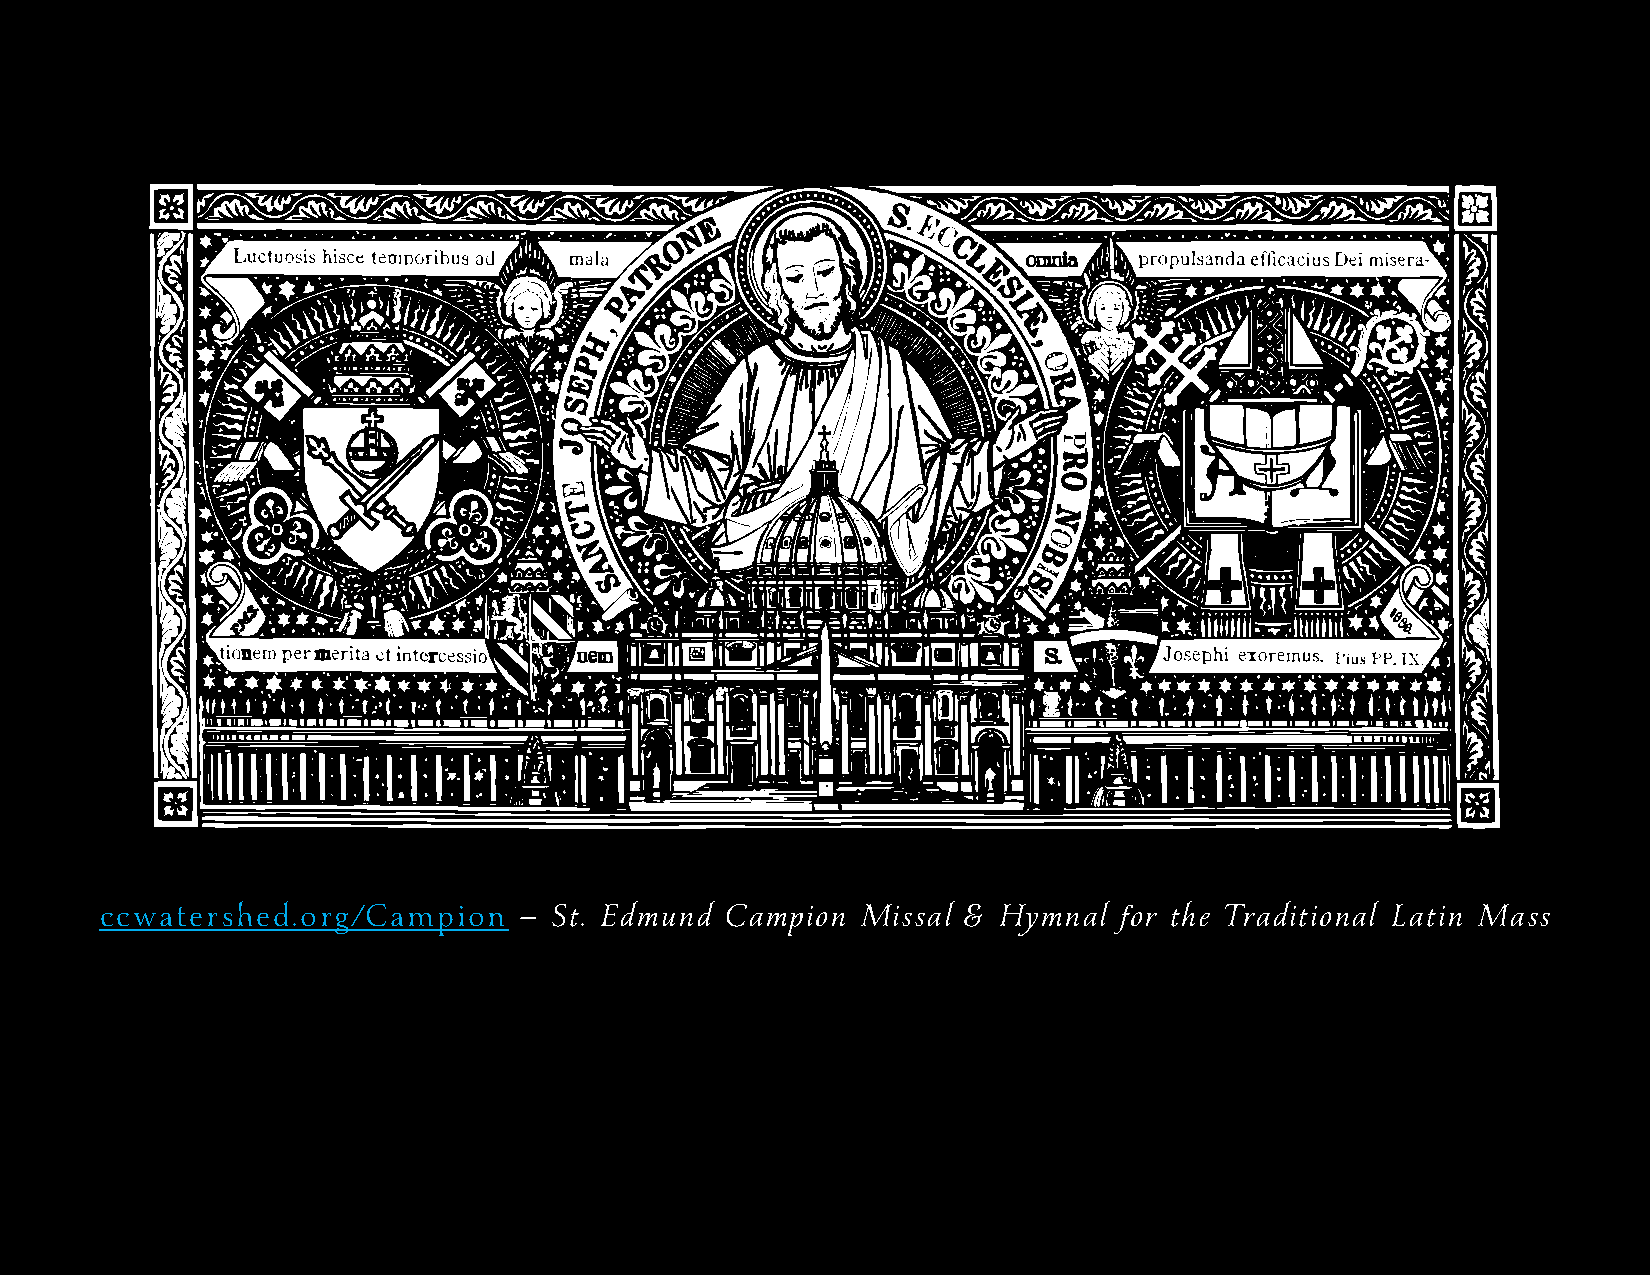
\includegraphics[clip,trim=0.98in 2.945in 0.99in 1.205in,width=0.91\textwidth]{../199_clipart.pdf}

\vfill

\end{centering}

\garamondbig
\greannotation{Hymn.}
\greannotation{1.}
\gregorioscore{200_hy--te_joseph_celebrent--solesmes}

\bigskip

\pagebreak

\gresetinitiallines{0}
\gregorioscore{202-vr-ora_pro_nobis}

\bigskip

\begin{centering}

\vfill

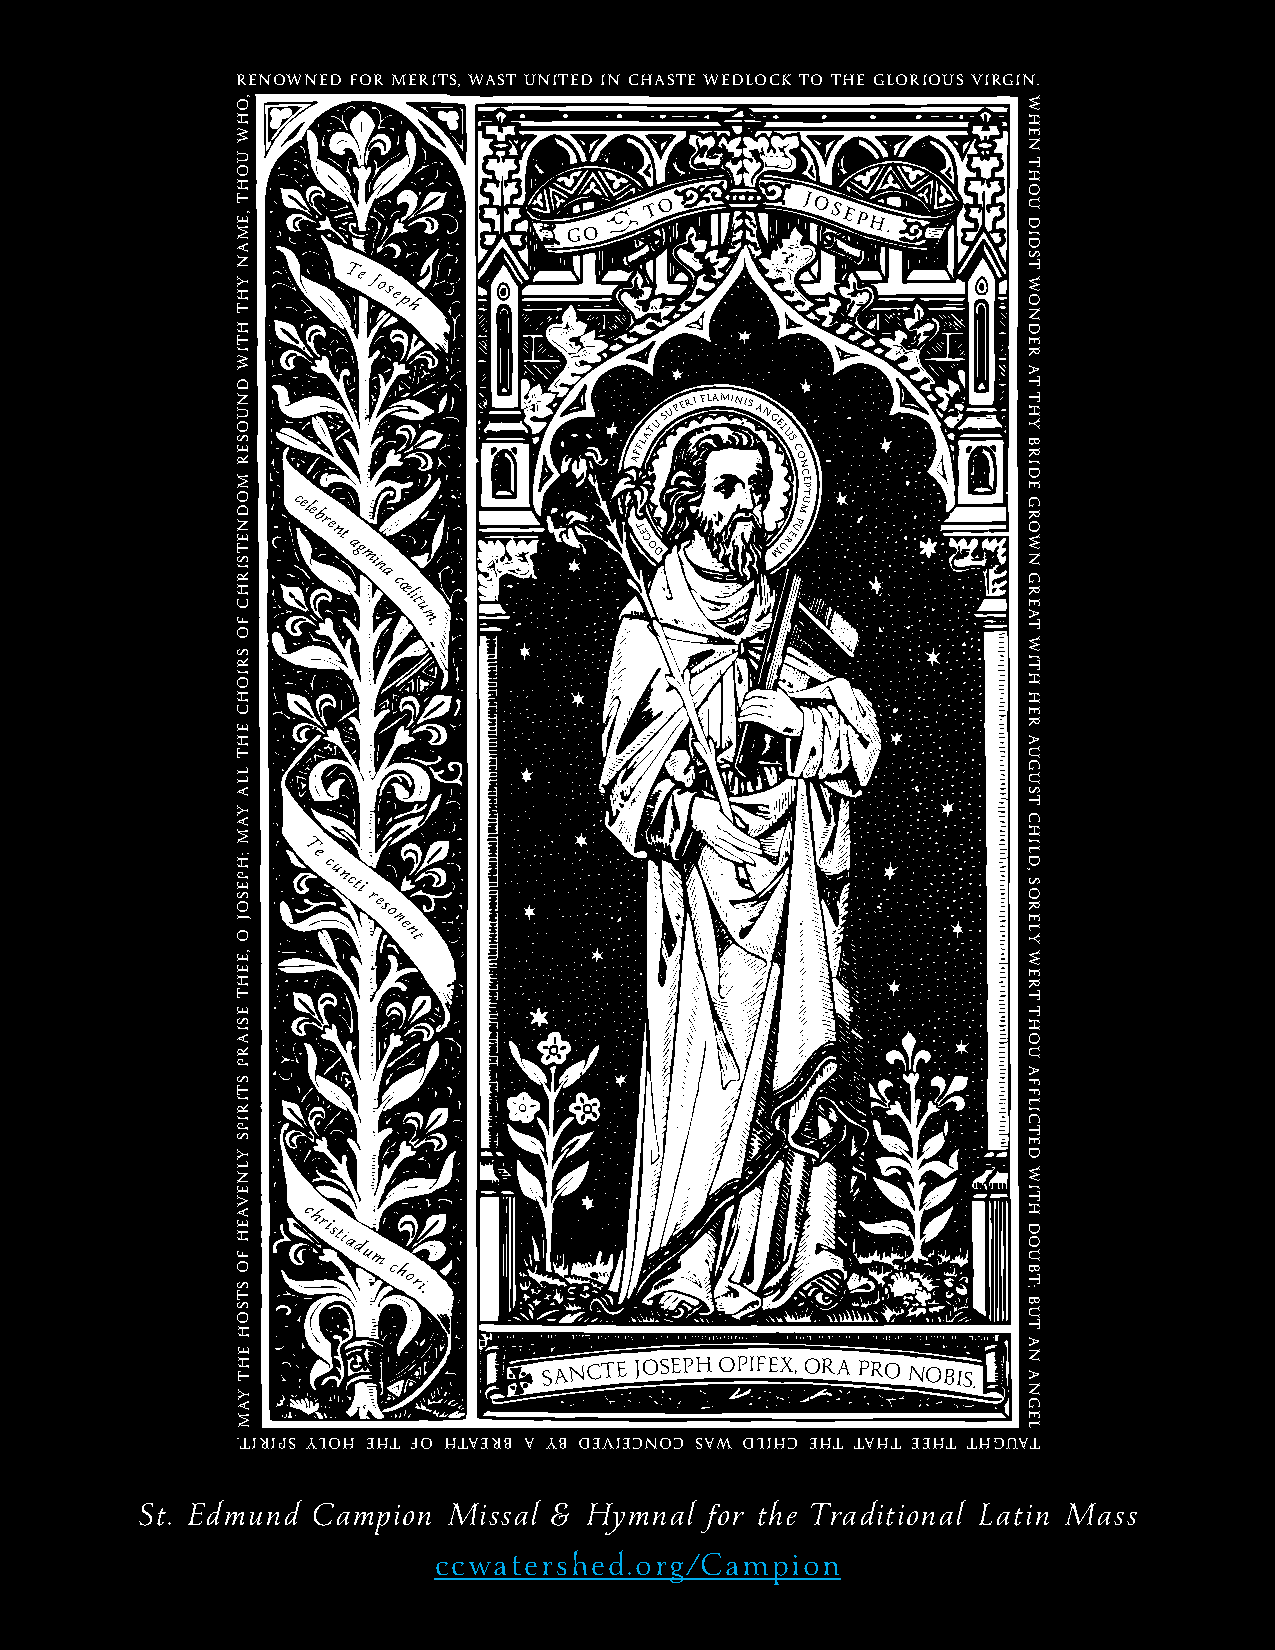
\includegraphics[clip,trim=1.706in 1.47in 1.708in 0.622in,width=0.53\textwidth]{../202_clipart.pdf}

\vfill

\end{centering}


\end{document}